\documentclass[12pt]{article}

\usepackage[T1]{fontenc}
\usepackage[polish]{babel}
\usepackage[utf8]{inputenc}
\usepackage{lmodern}
\selectlanguage{polish}

\usepackage{graphicx}
\usepackage{tabularx, booktabs}
\usepackage{fancyhdr} 
\usepackage{geometry}
\usepackage{hyperref}
\usepackage{listings}
\usepackage{float} 
\usepackage{subfigure}

\usepackage{a4wide}

\geometry{left=15mm,right=25mm,%
bindingoffset=10mm, top=20mm, bottom=20mm}
 


\renewcommand{\maketitle}{
\begin{titlepage}
\begin{table}[t]
\centering
\begin{tabular}[t]{lcr}
 
\includegraphics[width=70pt,height=70pt]{PW} & POLITECHNIKA WARSZAWSKA & 
\includegraphics[width=70pt,height=70pt]{MiNI}\\
& WYDZIAŁ MATEMATYKI & \\
& I NAUK INFORMACYJNYCH &
\end{tabular}
\end{table}
\vspace*{3cm}
  \begin{center}
    \LARGE
    \textbf {Raport}\\
   \vspace*{2 cm}
\begin{table}[!htp]
\begin{tabular}{p{4cm}p{10cm}}
\textit{Przedmiot:} &\textbf {Analiza i rozpoznawanie danych obrazowych} \\
\\
\textit{Projekt:} &\textbf {Zliczanie filtrów papierosowych} \\
\\
\textit{Autorzy:} &\textbf {Sebastian~Sudra \newline Łukasz~Sznajder \newline Nikodem~Wiśniewski} \\
\\
\end{tabular}
\end{table}

\vspace{5 cm}
  \center{\small Warszawa, dnia \today}
\end{center}
\end{titlepage}
}

\begin{document}
\maketitle

\newpage

\section{Opis projektu}
Zadaniem tego projektu jest obliczenie liczby filtrów papierosowych widocznych na zdjęciach będących plikami wejściowymi programu (Rysunek \ref{input}). Jako wyjście program wypisuje w konsoli liczbę zliczonych filtrów oraz tworzy plik z oznaczonymi filtrami na obrazie wejściowym.


\begin{figure}[H]
\centering 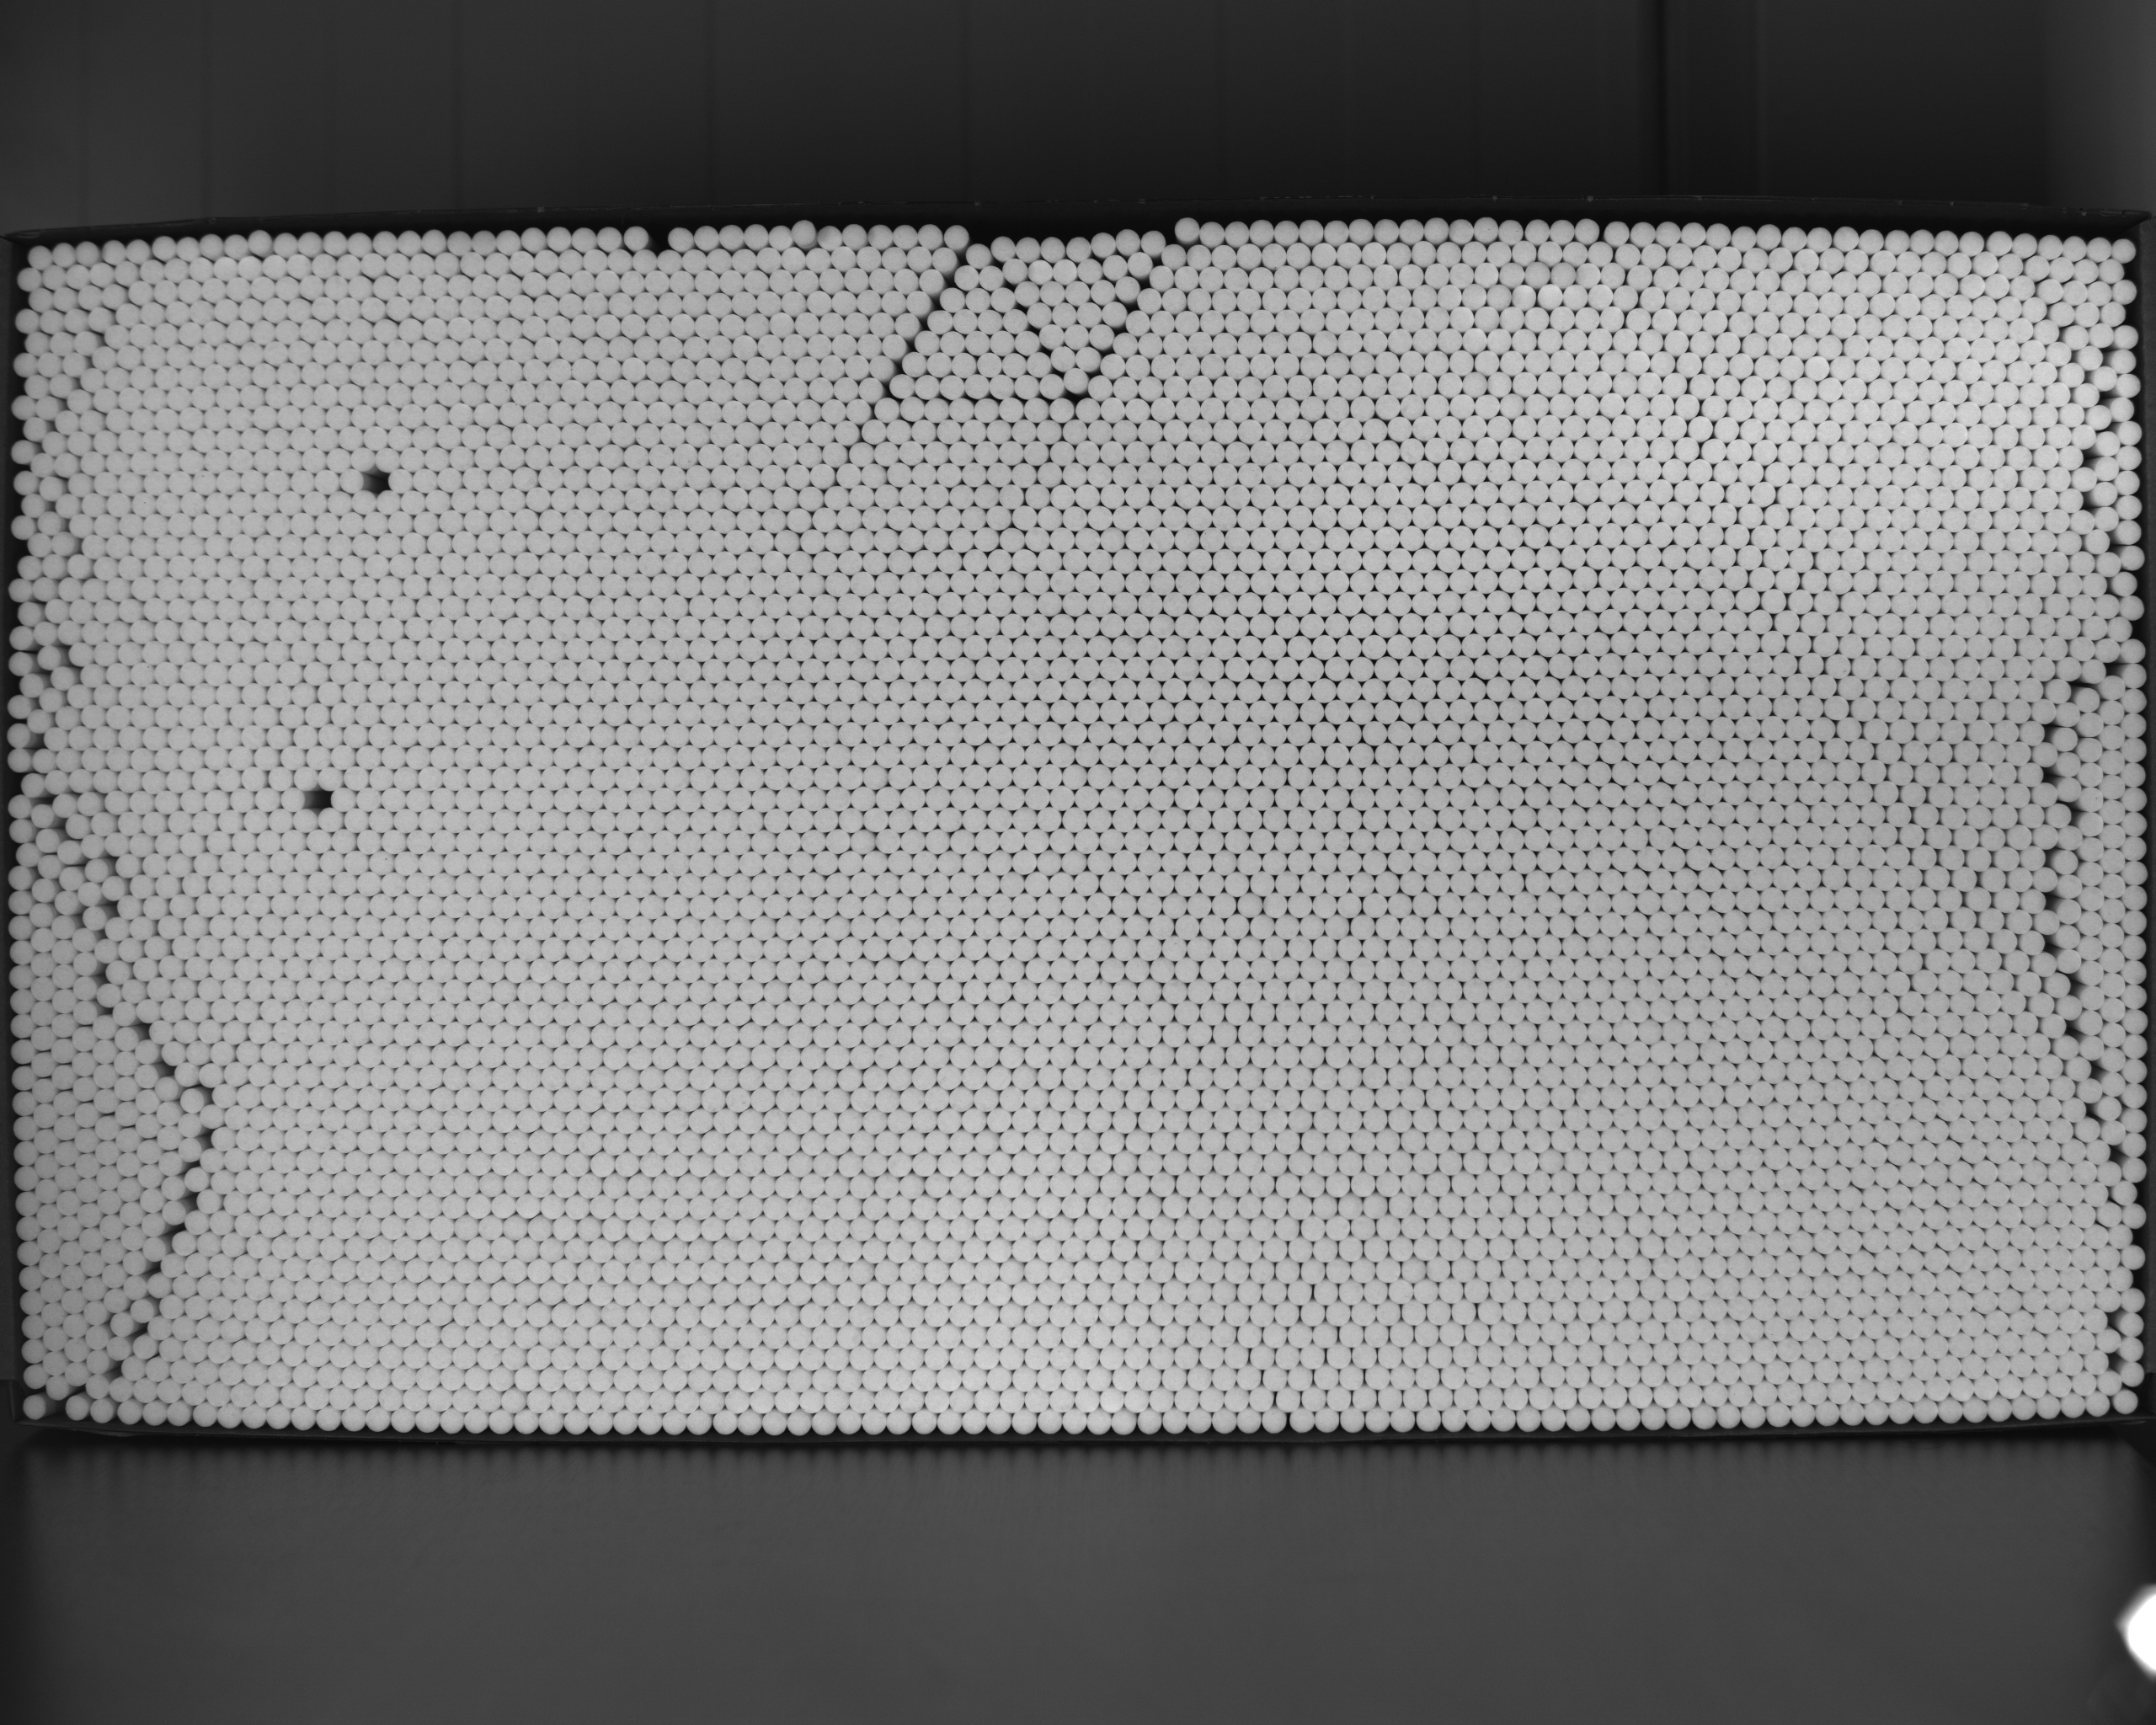
\includegraphics[scale=0.3]{1.png}
\caption{Obraz wejściowy}
\label{input}
\end{figure}

\section{Algorytm}
Algorytm skłąda się z dwóch głównych faz: fazy preprocessingu oraz z fazy wykrywania okręgów.

\subsection{Rozmycie gaussowskie}
Przed rozpoczęciem głównych operacji, wejściowy obraz ulega operacji rozmycia w celu usunięcia drobnych szumów mogących zakłócić wykrywanie filtrów.


\begin{figure}[H]
\centering 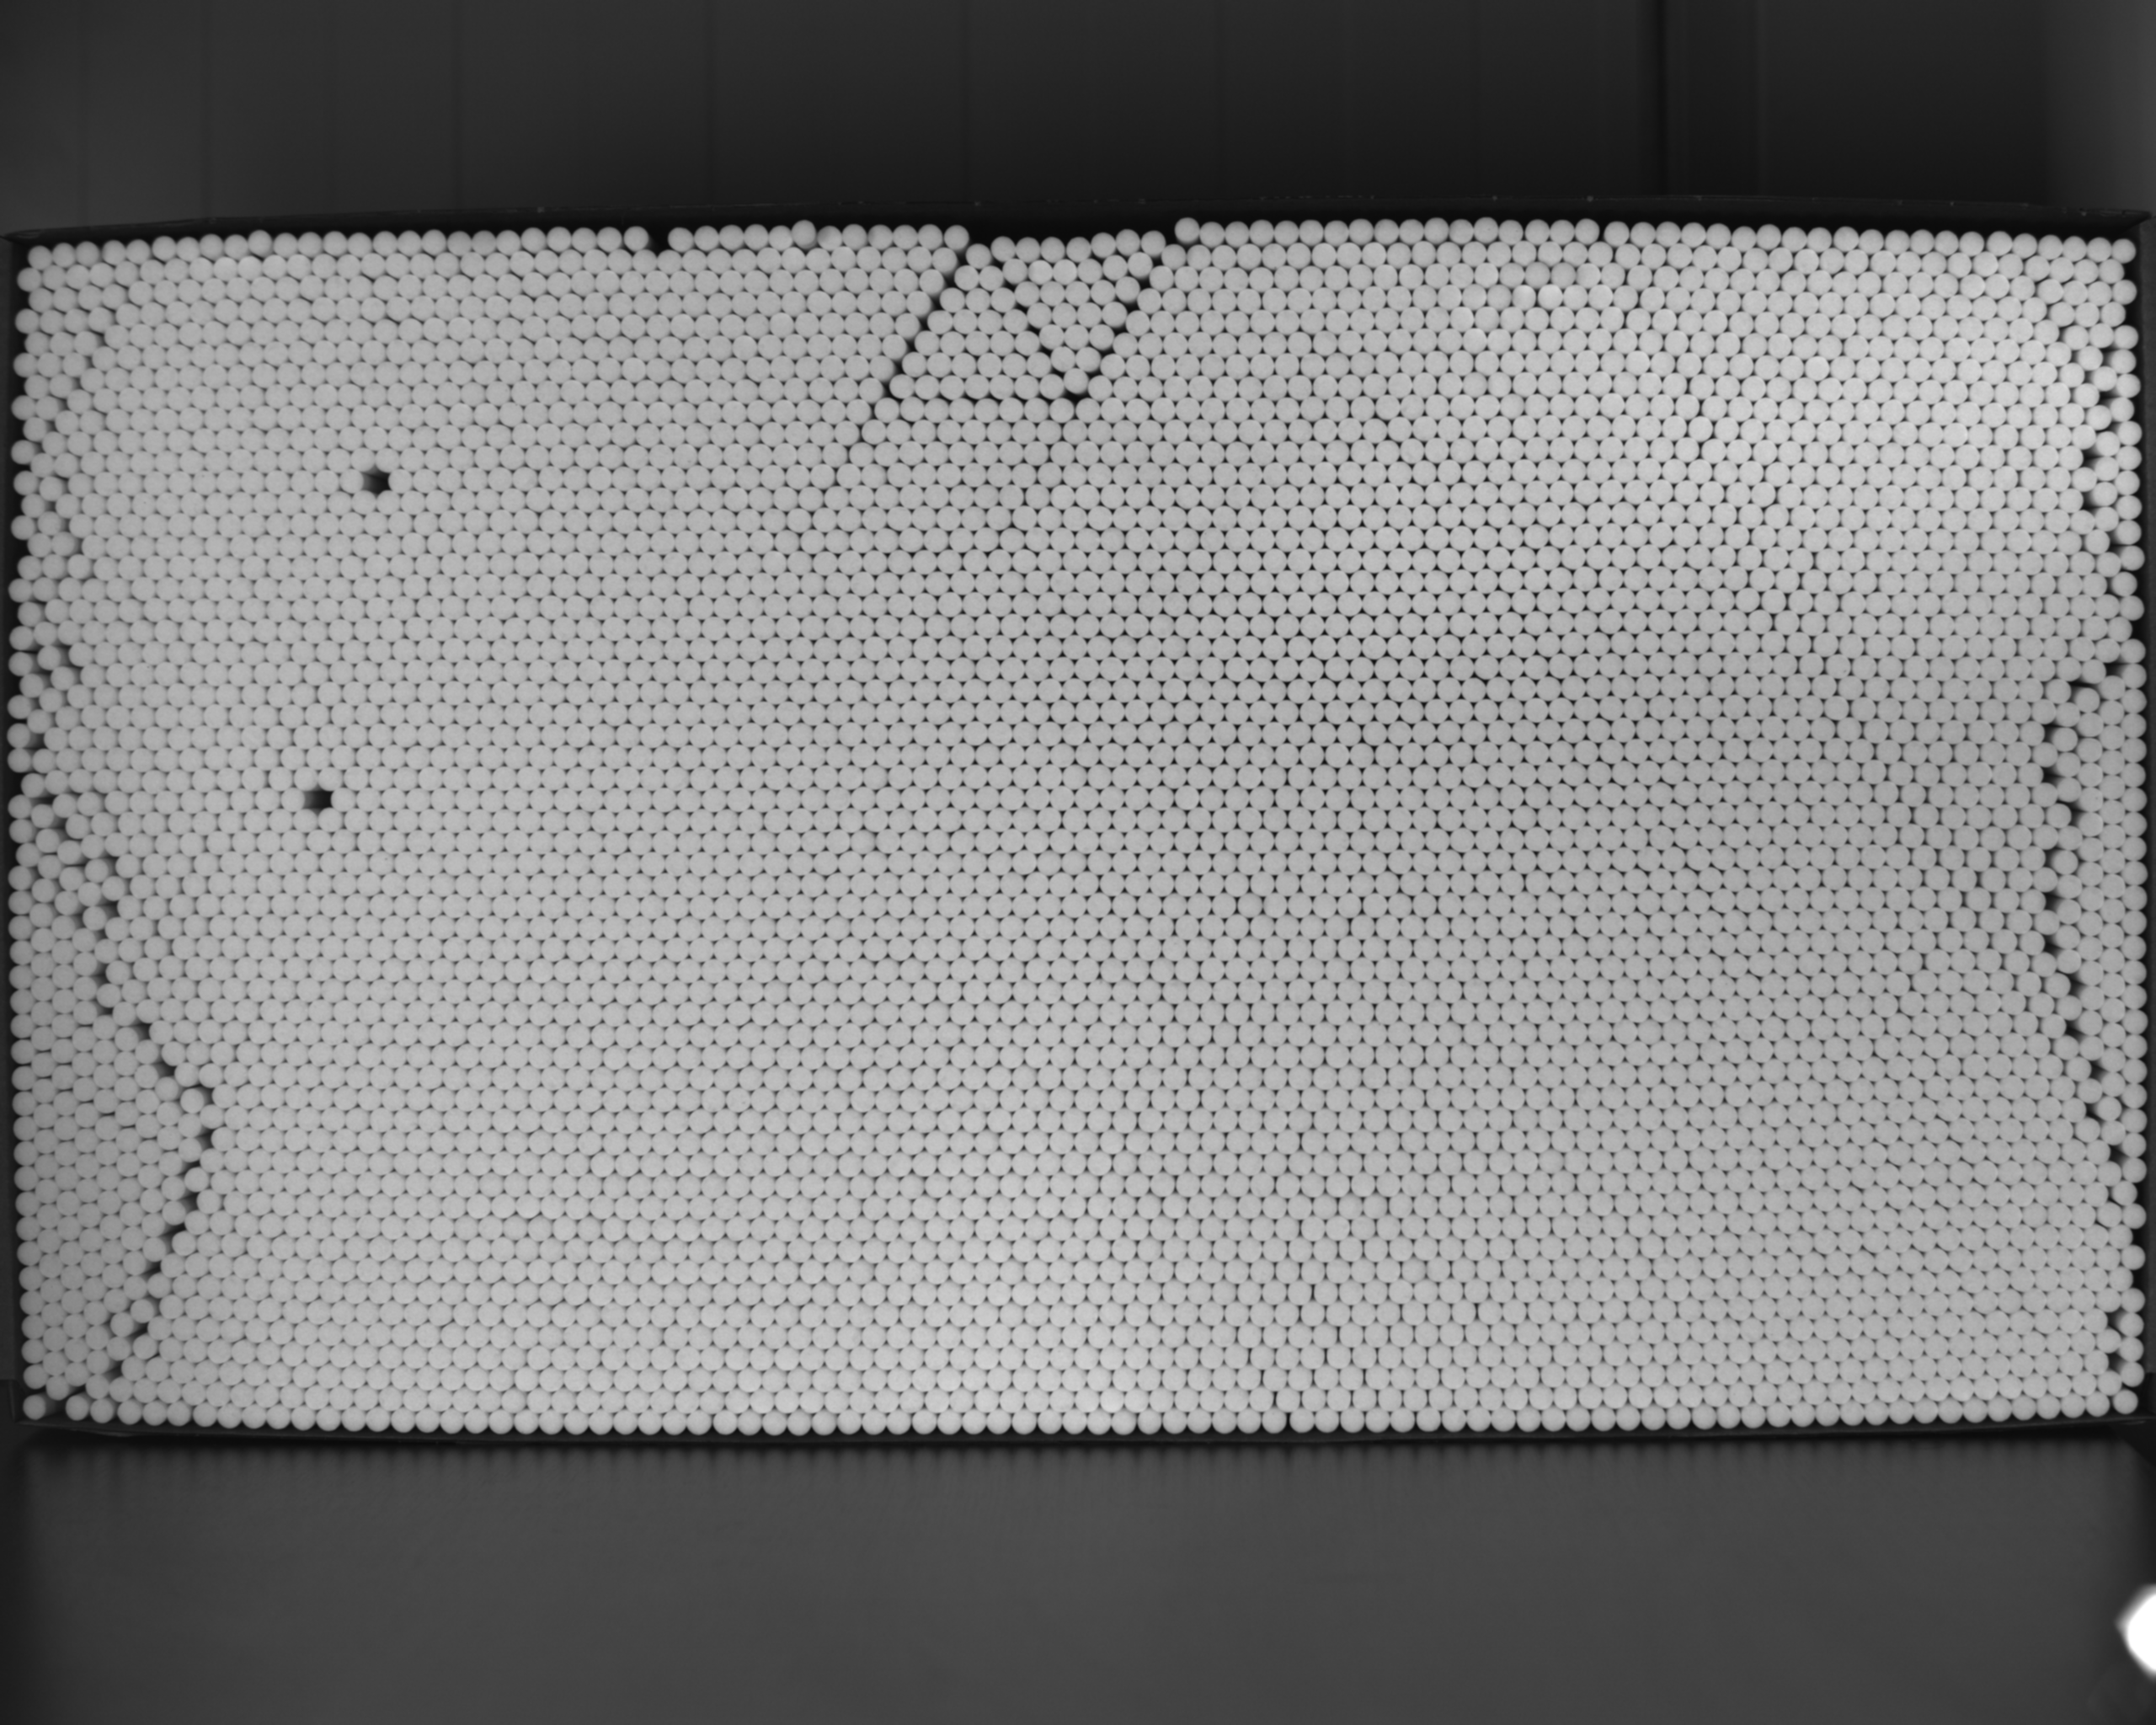
\includegraphics[scale=0.108]{step1.png}
\caption{Obraz rozmyty}
\label{blur}
\end{figure}

\subsection{Segmentacja obrazu}

W celu wyeliminowania marginesów widocznych z góry oraz dołu Rysunku \ref{blur} stosowany jest obraz maska. Obraz maska uzyskiwany jest poprzez binaryzację z progiem globalnym.

\begin{figure}[H]
\centering 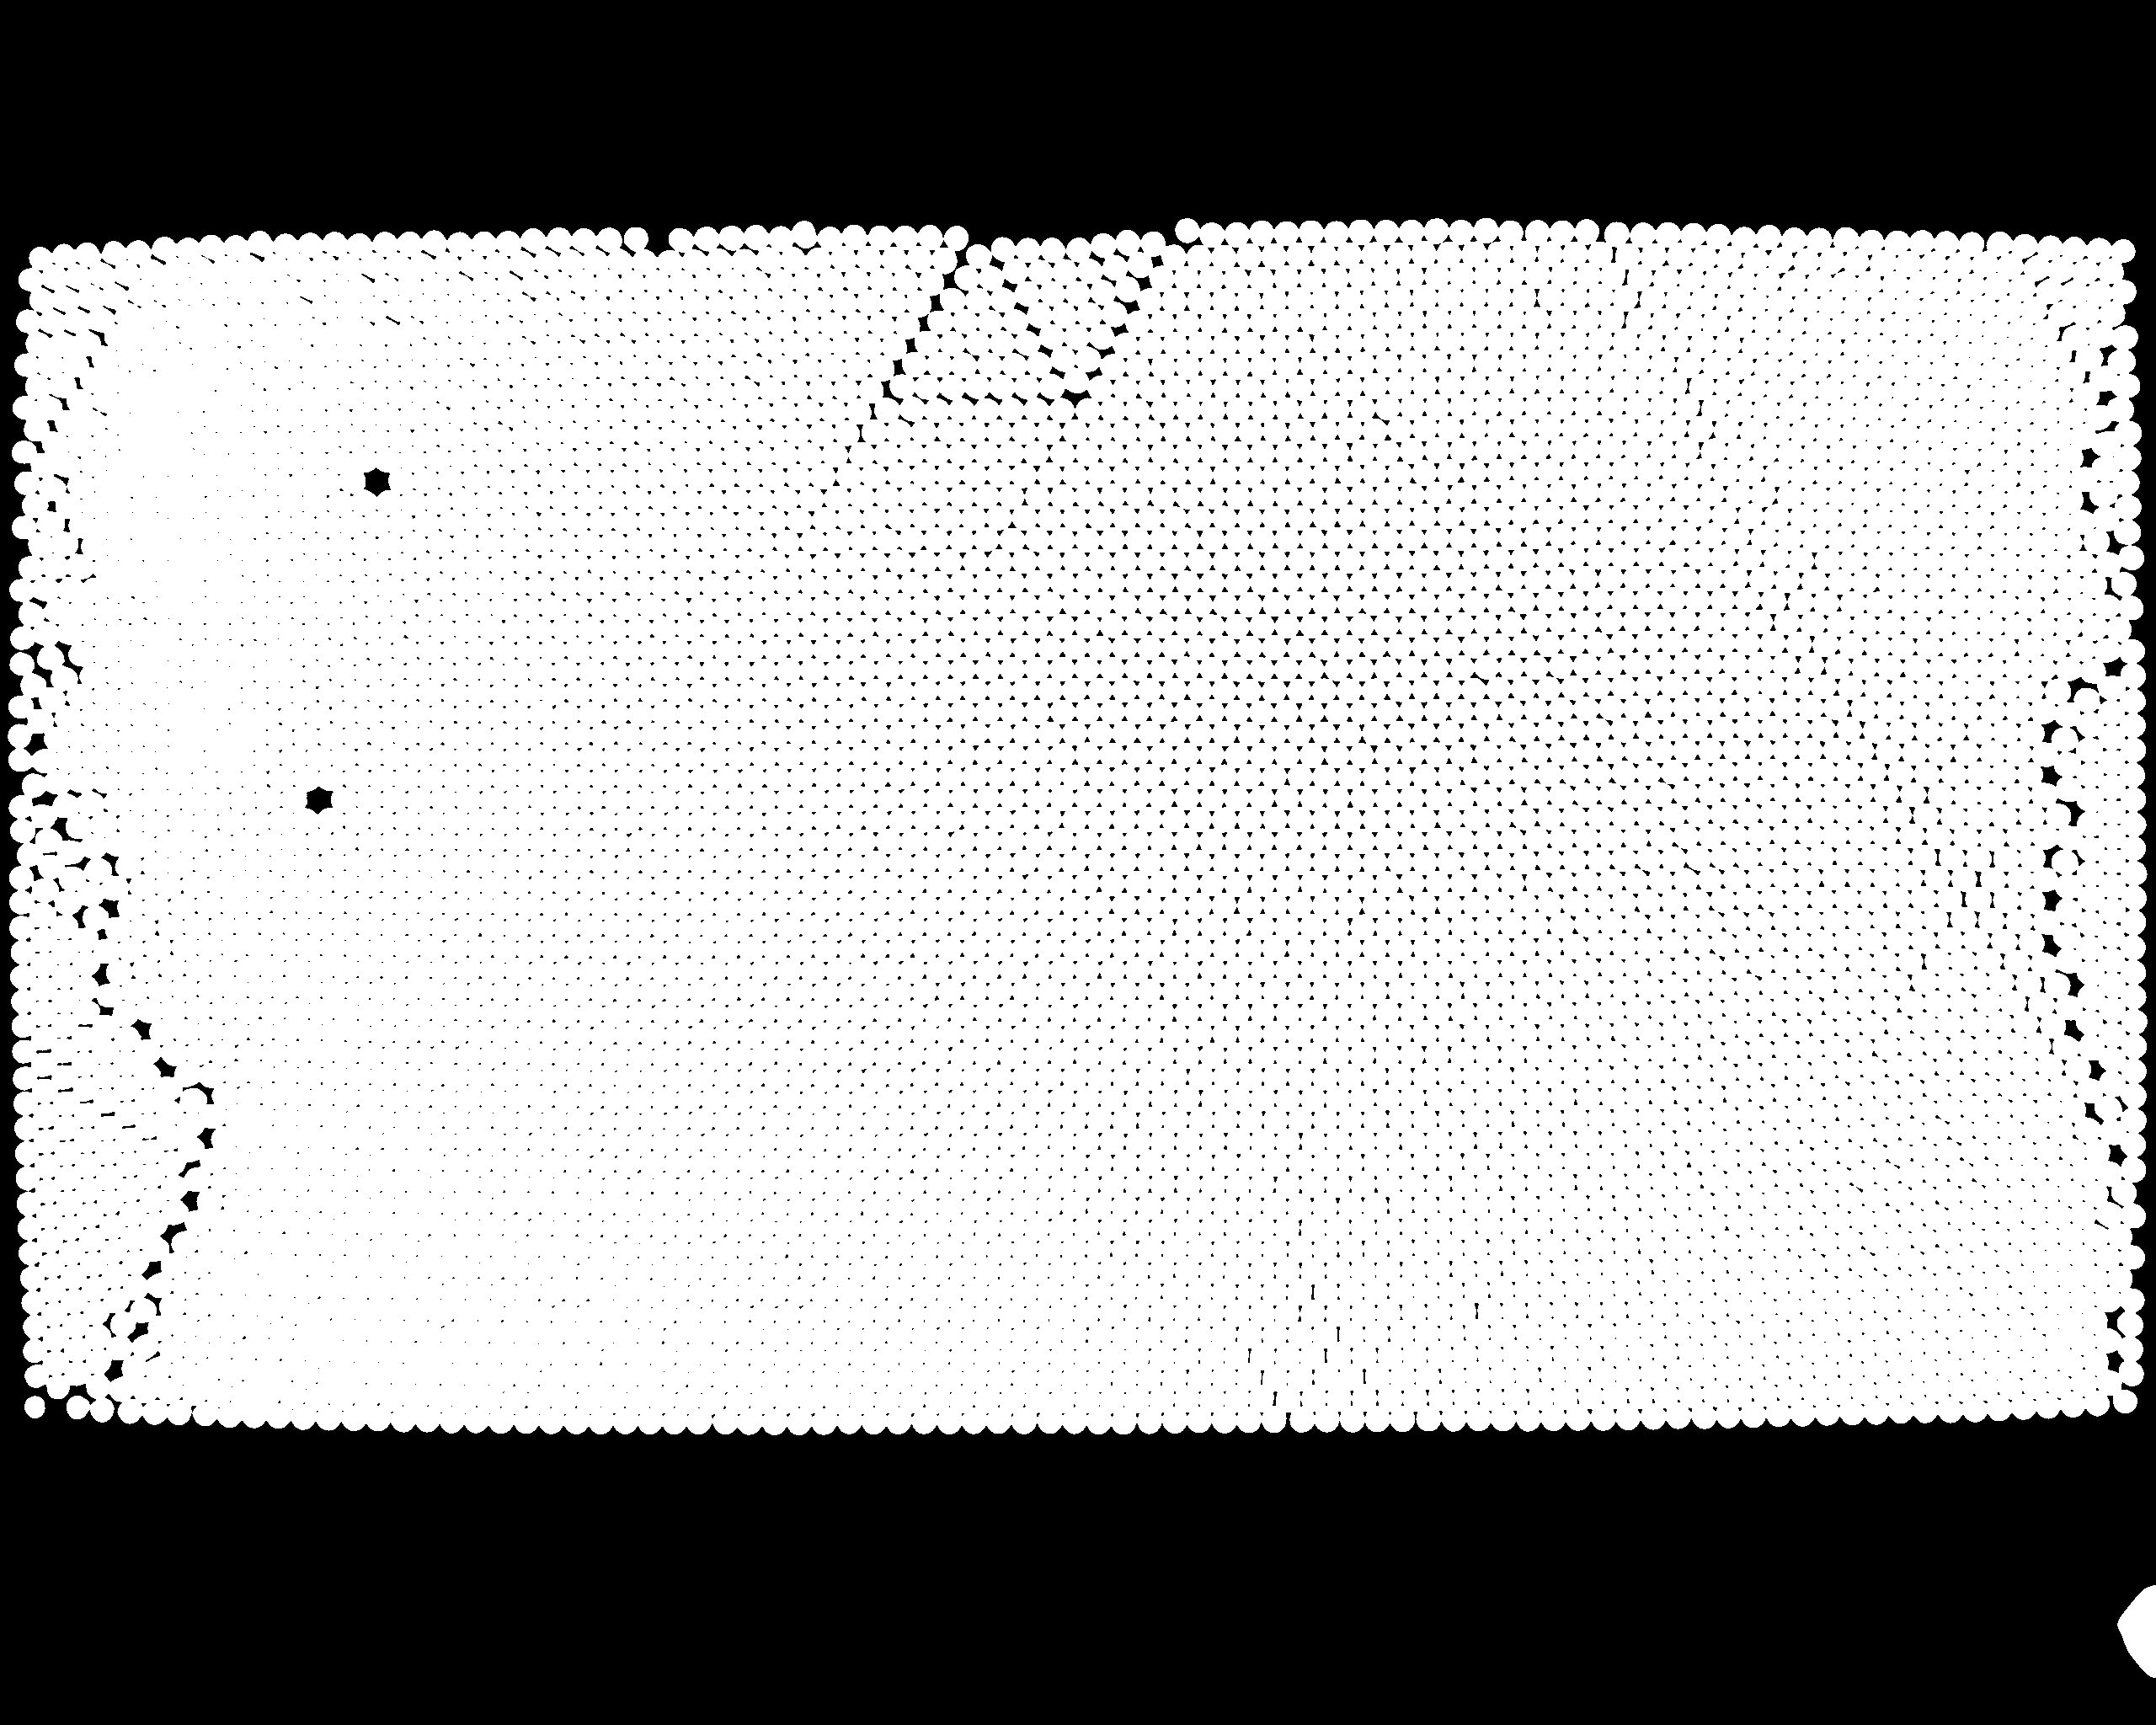
\includegraphics[scale=0.108]{step2.png}
\caption{Obraz pomocniczy - maska}
\label{reduct}
\end{figure}

Na obraz z poprzedniego kroku (Rysunek \ref{blur}) nakładane są wszystkie czarne piksele z Rysunku \ref{reduct} dzięki czemu uzyskiwana jest segmentacja obrazu wejściowego. Wynik widoczny jest na Rysunku \ref{segmented}.

\begin{figure}[H]
\centering 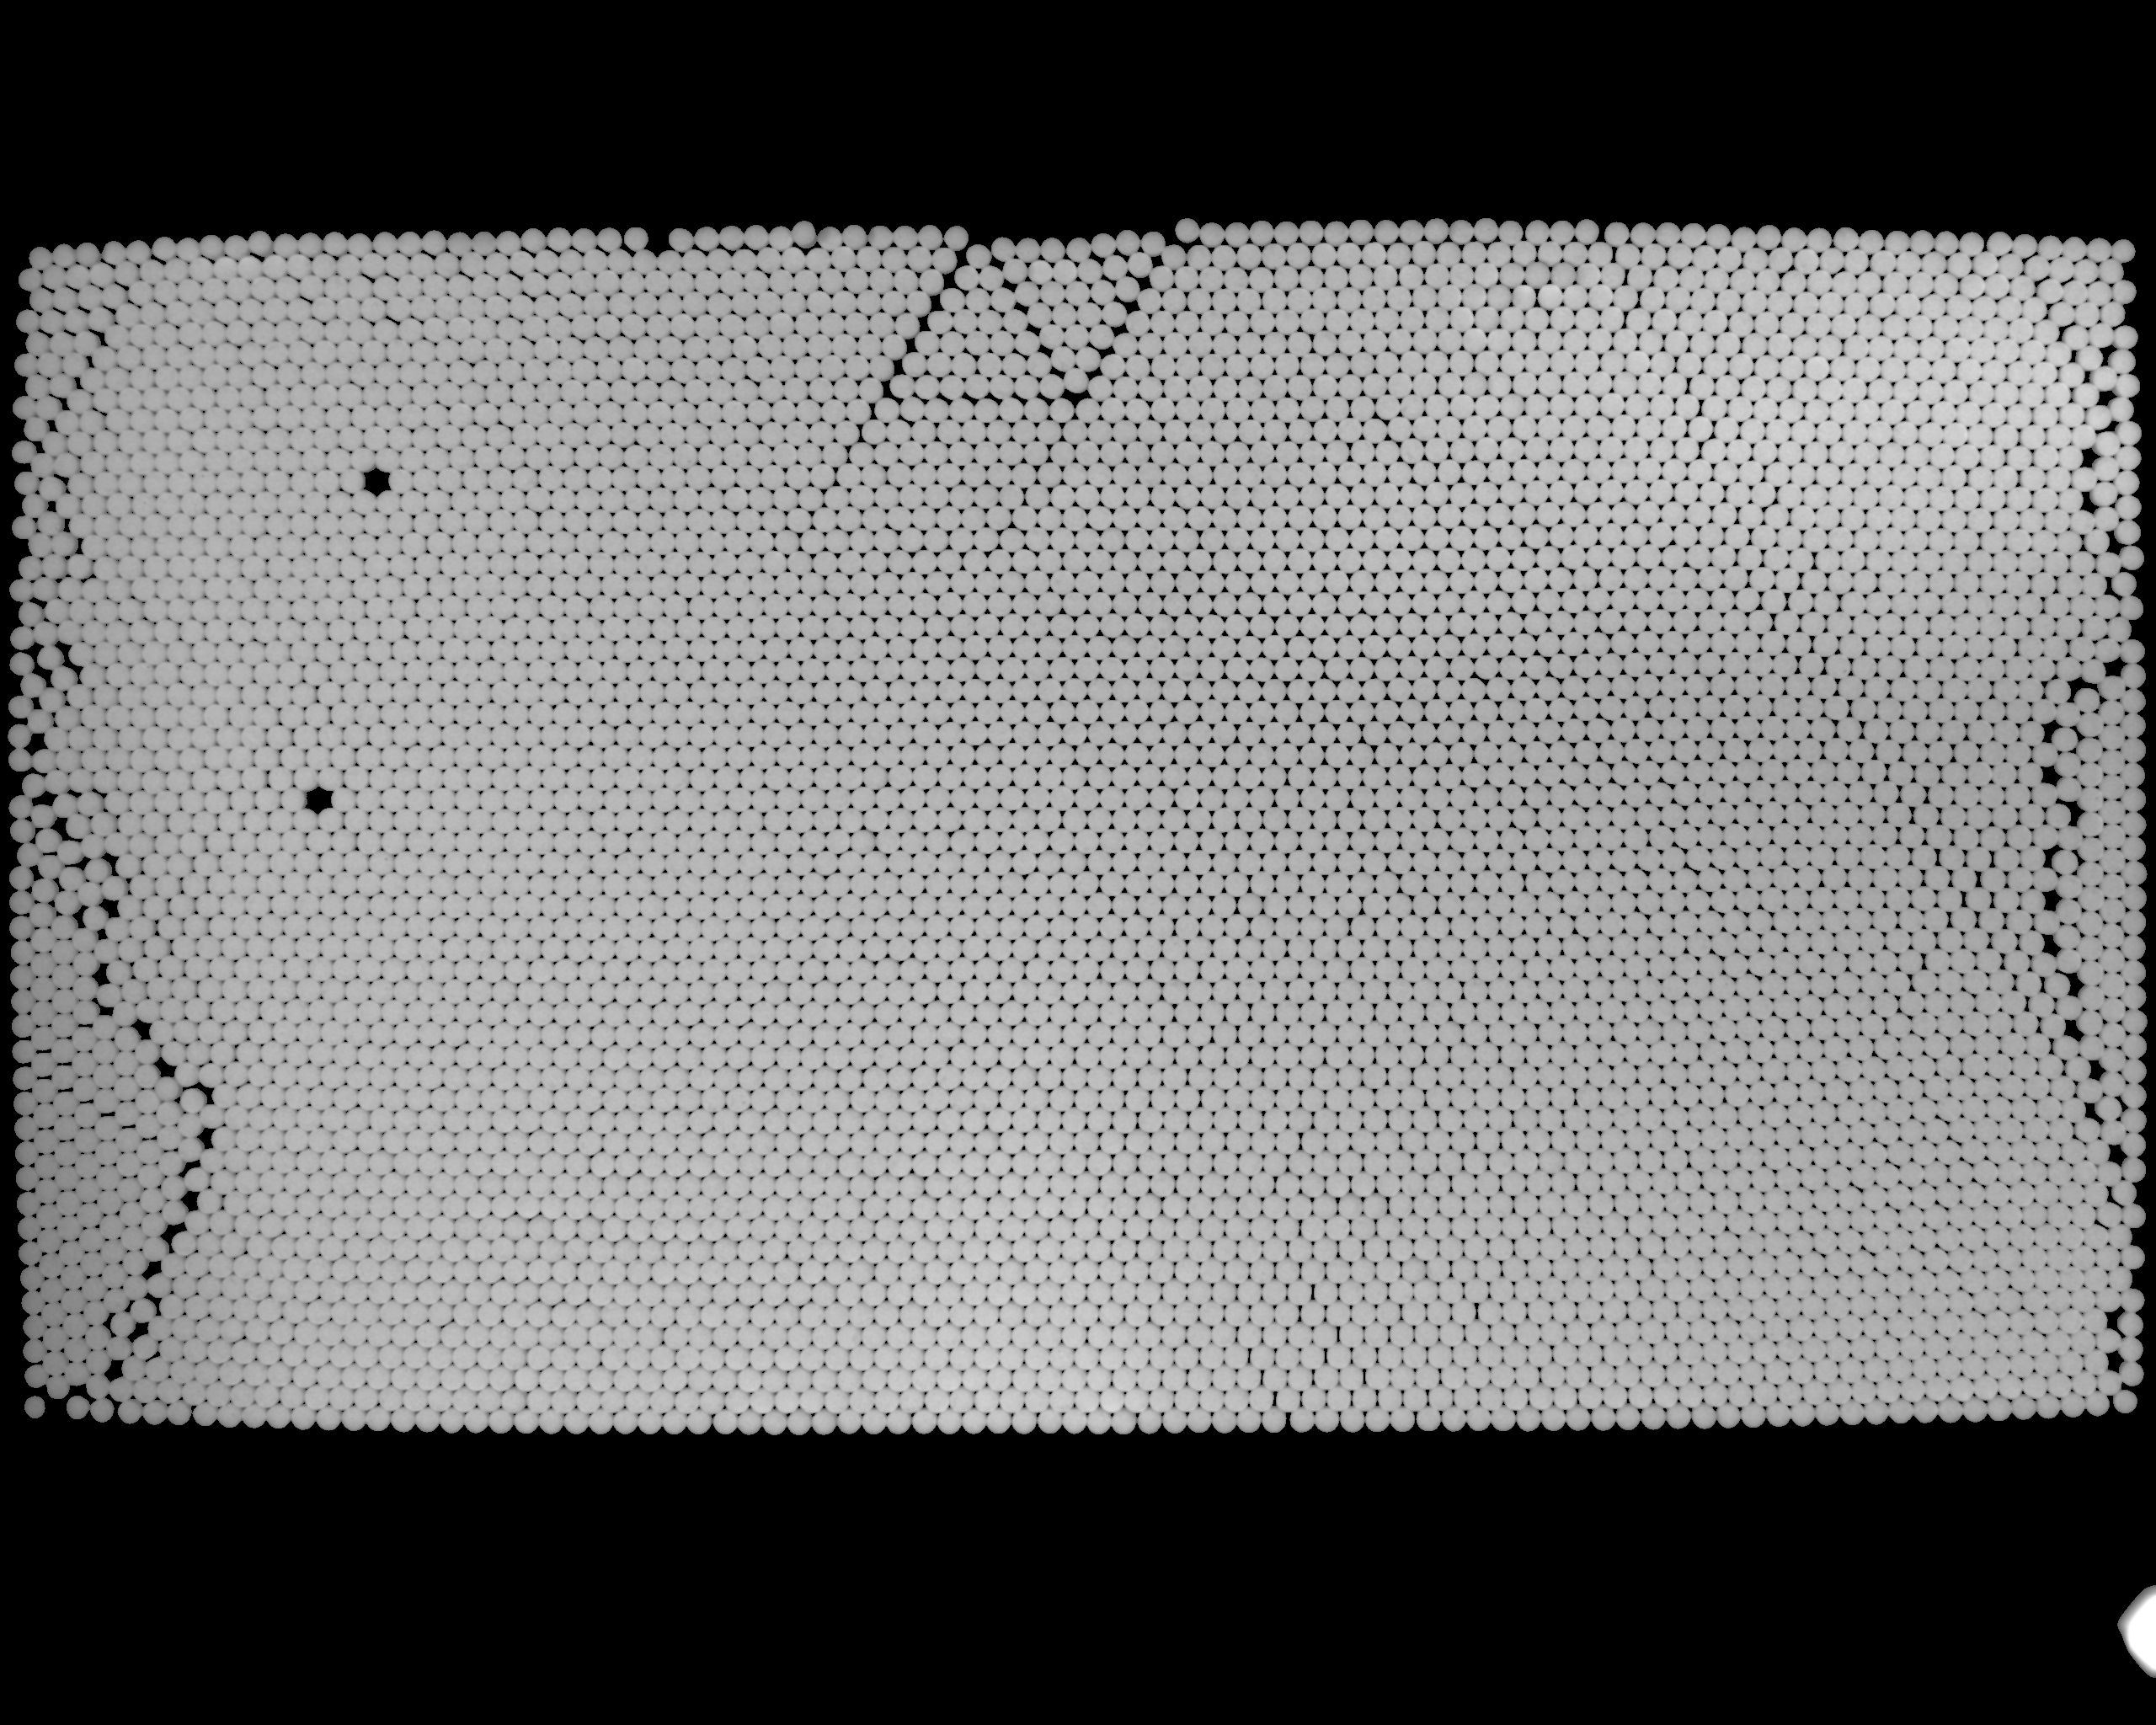
\includegraphics[scale=0.108]{step3.png}
\caption{Obraz po segmentacji}
\label{segmented}
\end{figure}

\subsection{Binaryzacja}
Na otrzymany zsegmentowanym obrazie wykonywana jest binaryzacja z progriem lokalnym (\textit{adaptive Gaussian threshold}).

\begin{figure}[H]
\centering 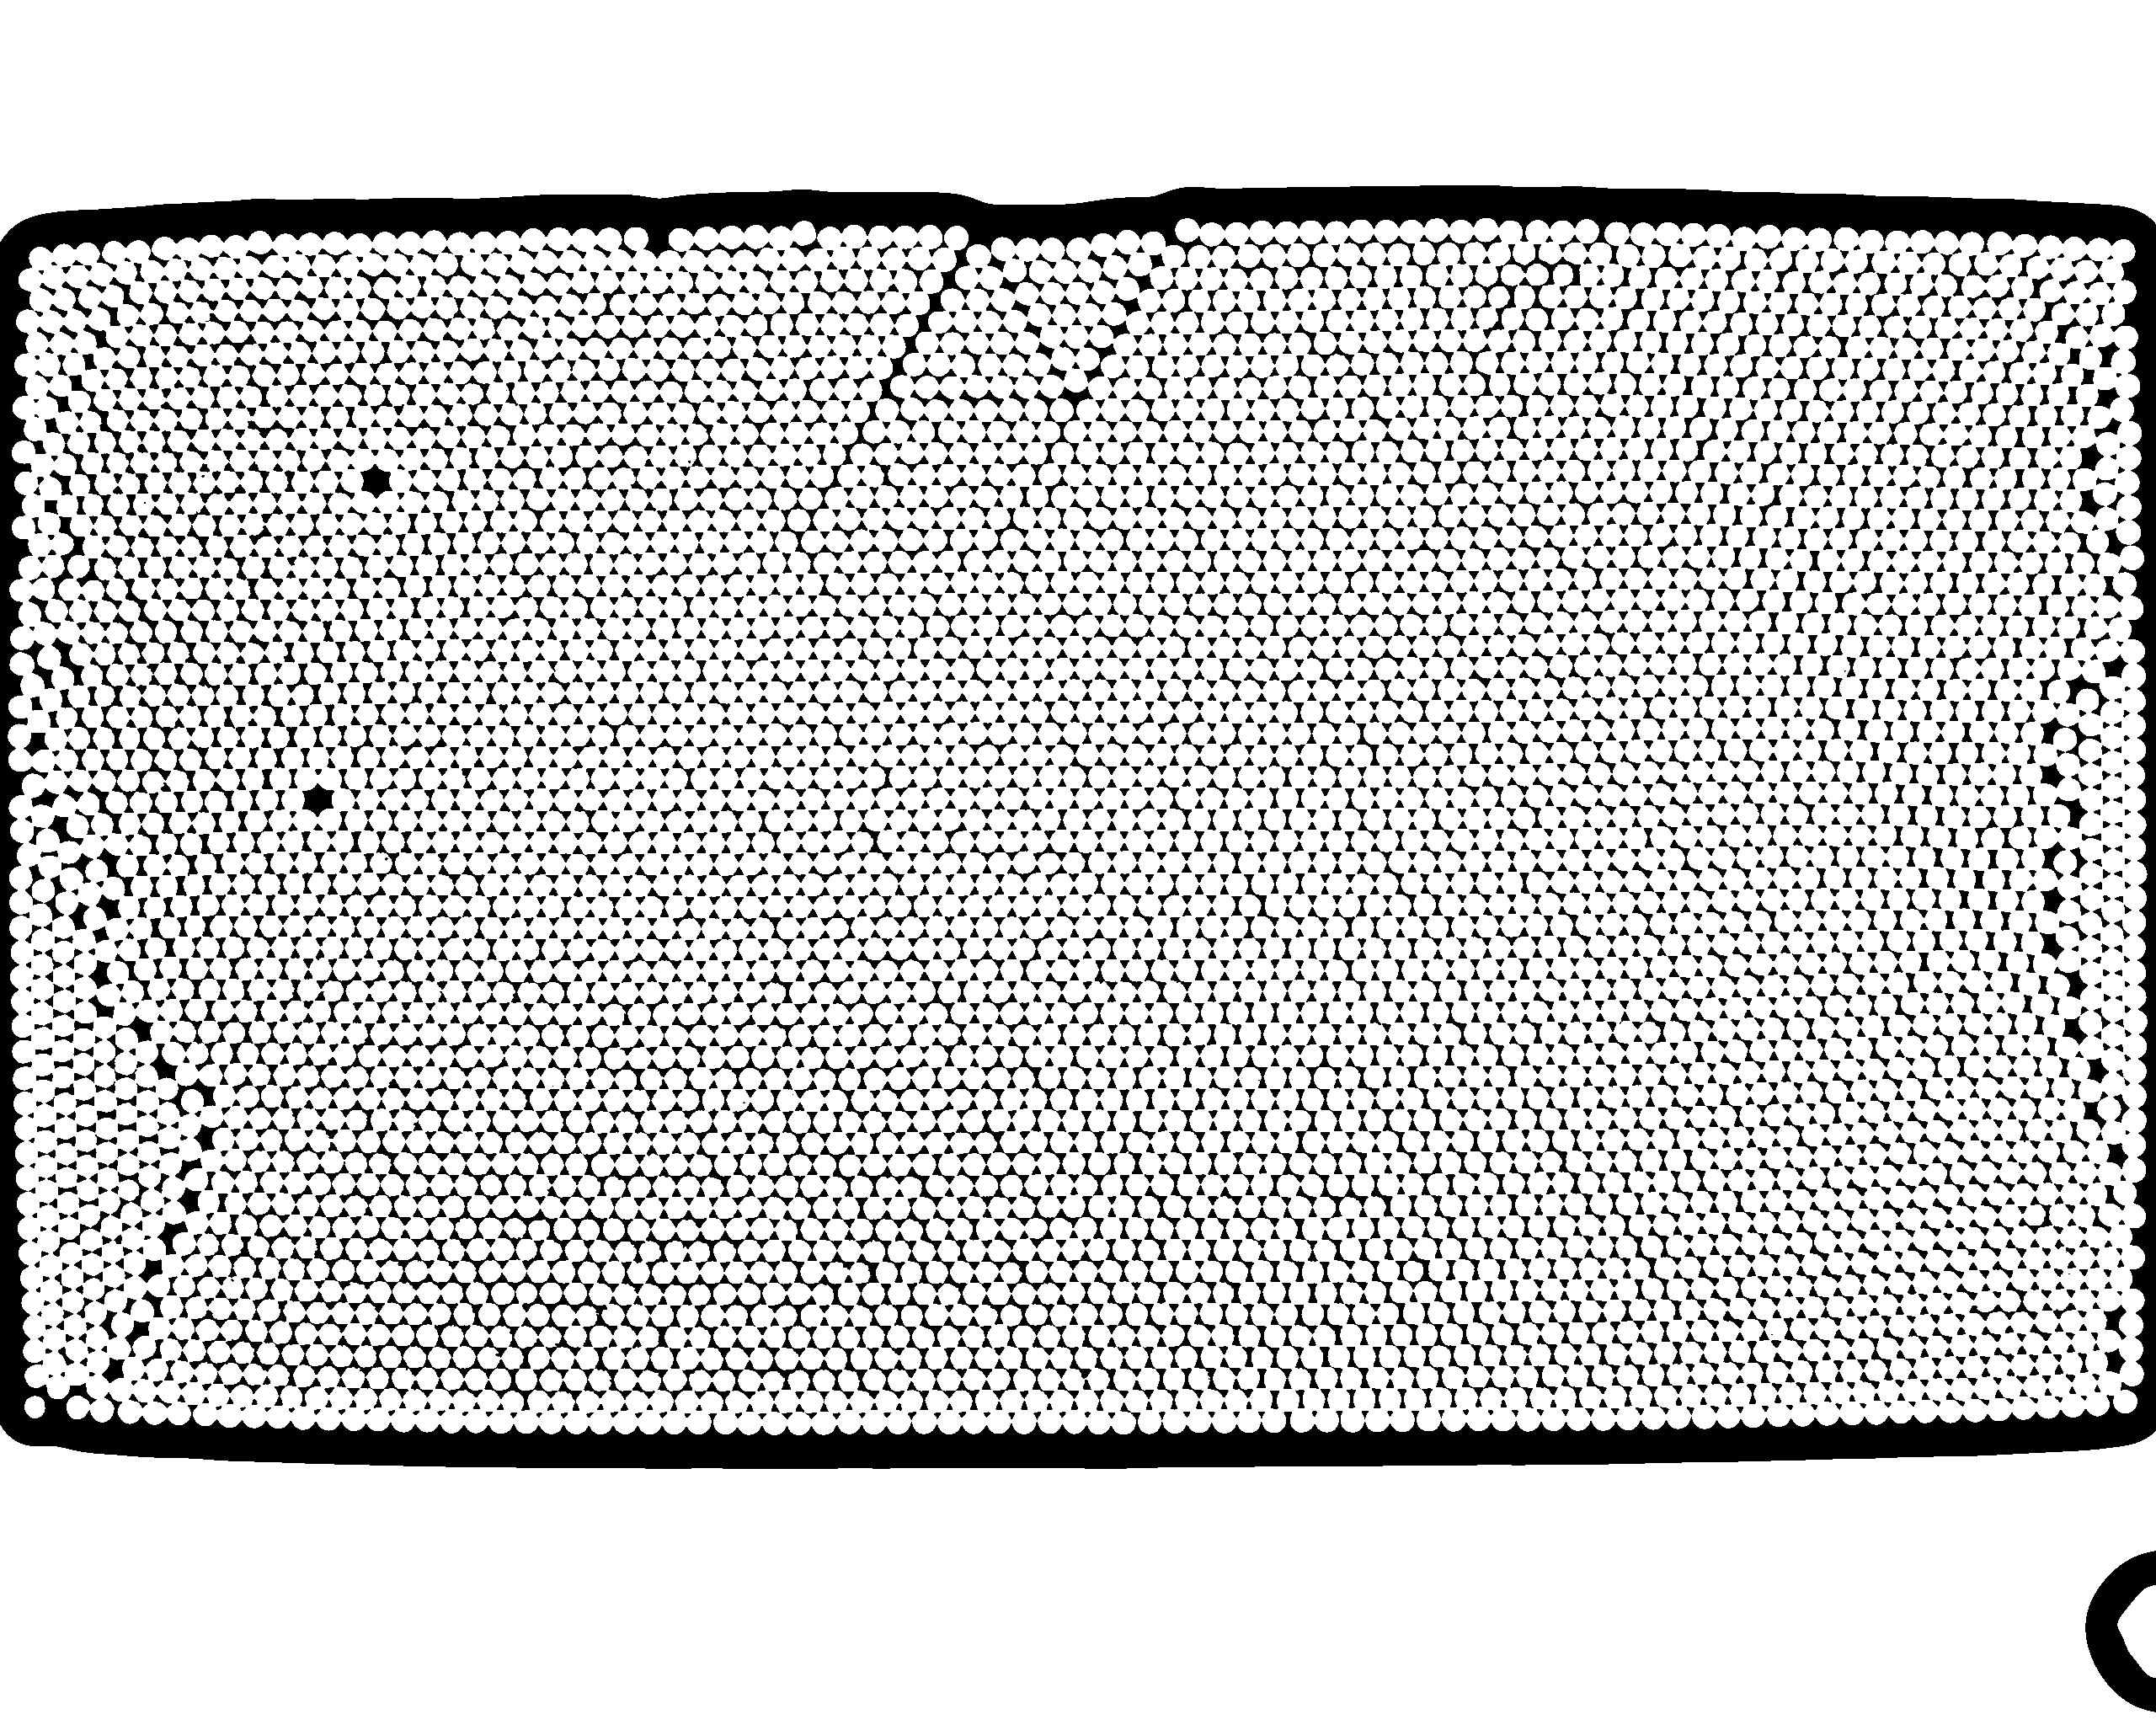
\includegraphics[scale=0.108]{step4.png}
\caption{Obraz po binaryzacji lokalnej}
\label{binary}
\end{figure}

\subsection{Wykrywanie krawędzi}
Po zbinaryzowaniu obrazu wejściowego następuje wykrywanie krawędzi metodą \textit{Canny'ego}.

\begin{figure}[H]
\centering 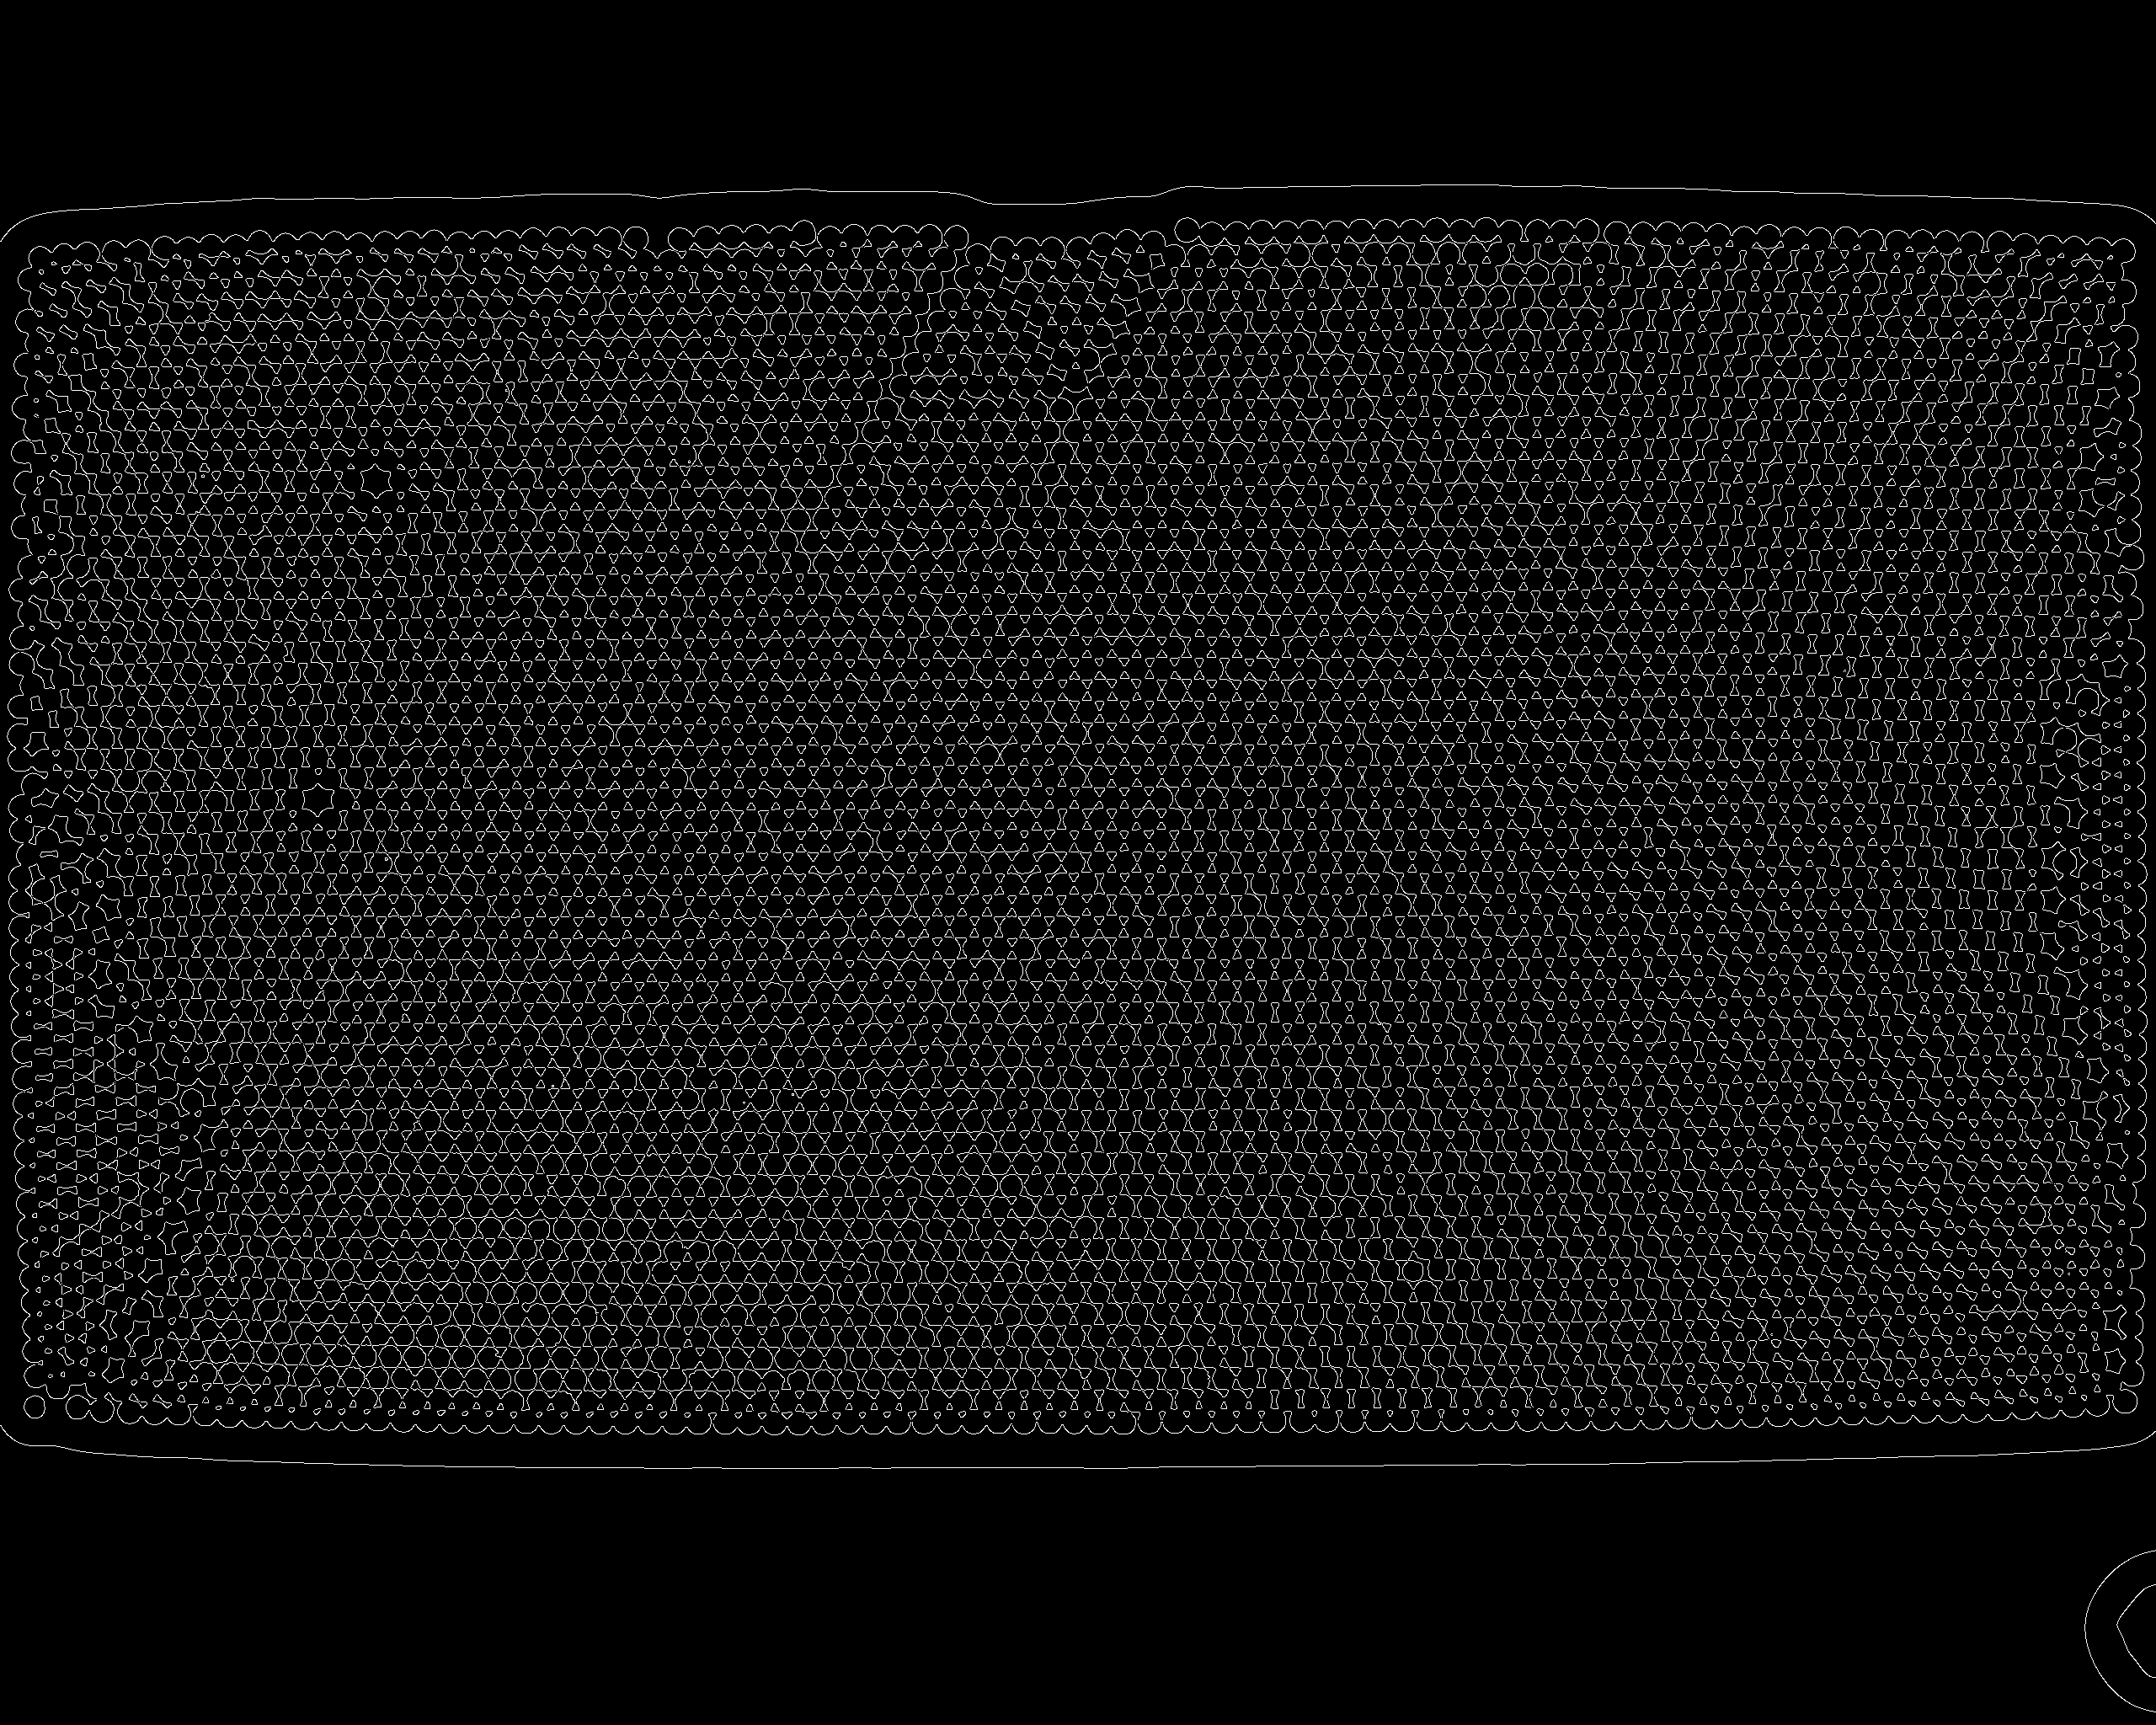
\includegraphics[scale=0.108]{step5.png}
\caption{Obraz z wykrytymi krawędziami}
\label{edges}
\end{figure}

\subsection{Transformacja Hough}
Po wykryciu wszystkich krawędzi algorytm przechodzi do wykrycia okręgów transformacją \textit{Hough}. Rysnuek \ref{circles} przedstawia obraz wejściowy z nałożonymi czarnymi okręgami ze środkiem oznaczonym na czerwono, w miejscach gdzie algorytm wykrył okrąg.

\begin{figure}[H]
\centering \includegraphics[scale=0.108]{step6.png}
\caption{Obraz z wykrytymi okręgami}
\label{circles}
\end{figure}

\subsection{Postprocessing}
Jak widać na Rysunku \ref{fail} algorytm nie jest w stanie odróżnić filtra od luki powstałej pomiędzy papierosami gdy ma ona okrągły kształt.

Z tego powodu po wykryciu wszystkich okręgów dodana jest faza, podczas której odrzucane są wszystkie te okręgi, których środek wypada w miejscu ciemnego piksela. Wynik widoczny jest na Rysunku \ref{fix}.

\begin{figure}[H]%
\centering
\subfigure[Obraz z nadmiarowymi okręgami]{%
\label{fail}
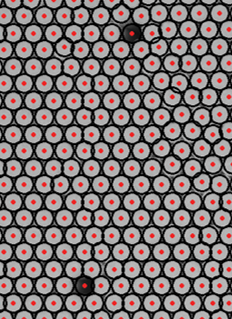
\includegraphics[scale=0.7]{fail.png}}%
\qquad
\subfigure[Obraz bez nadmiarowych okręgów]{%
\label{fix}
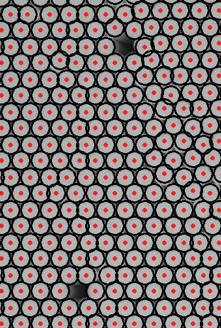
\includegraphics[scale=0.7]{fix.png}}%
\caption{Nadmiarowe okręgi}
\end{figure}

\section{Instrukcja obsługi}

Program uruchamiany jest poprzez skrypt \textbf{program.py} napisany w języku \textit{Python 3.6}. Na początku skryptu są zadeklarowane dwa parametry sterujące wykonaniem programu:
\begin{itemize}
\item \textit{INPUT\_FILE\_PATH} ścieżka do pliku wejściowego;
\item \textit{SAVE\_EACH\_PROCESS\_STEP} flaga decydująca o zapisywaniu wszystkich pośrednich kroków wykonania programu.
\end{itemize}

Wynikiem programu jest widoczna w konsoli liczba znalezionych filtrów oraz czas wykonania programu. Dodatkowo program w miejscu uruchomienia skryptu tworzy plik wyjściowy z oznaczonymi filtrami na obrazie wejściowym o nazwie \textbf{circles.png}.

\section{Wyniki i wnioski}
Wyniki projektu zostały opracowane w oparciu o zbiór siedmiu unikalnych obrazów wejściowych. Każdy z obrazów został ręcznie przeanalizowany pod względem liczby filtrów dzięki czemu możliwa była ocena jakości zaimplementowanego programu.

\begin{figure}[H]%
\centering
\subfigure[4725 filtrów 100\%]{%
\includegraphics[scale=0.055]{circles1.png}}%
\qquad
\subfigure[4725 filtrów 100\%]{%
\includegraphics[scale=0.055]{circles2.png}}%
\qquad
\subfigure[4724 filtry 99.98\%]{%
\includegraphics[scale=0.055]{circles3.png}}%
\qquad
\subfigure[4753 filtry 100\%]{%
\includegraphics[scale=0.055]{circles4.png}}%
\qquad
\subfigure[4725 filtrów 100\%]{%
\includegraphics[scale=0.055]{circles5.png}}%
\qquad
\subfigure[4708 filtrów 100\%]{%
\includegraphics[scale=0.055]{circles6.png}}%
\qquad
\subfigure[4709 filtrów 99.98\%]{%
\includegraphics[scale=0.055]{circles7.png}}%

\caption{Wyniki programu}
\label{results1}
\end{figure}

Spośród dostępnych danych testowych uzyskaliśmy prawie 100\% dokładności. Na przedstawionych obrazach jest łącznie 33 071 filtrów z których program nie wykrył tylko dwóch. Daje to dokładność na poziomie 99.994\%. Warto zauważy, iż prosta operacja usuwania nadmiarowych okręgów pozwoliła na całkowite pozbycie się ich. Choć na obrazach wyjściowych widoczne są delikatne przesunięcia filtrów od znalezionych okręgów nie ma to żadnego wpływu na liczbę zliczonych obiektów. Uzyskany algorytm jest odporny na nierówne oświetlenie (Rysunek \ref{light}) co jego jest dodatkową zaletą. 

\begin{figure}[H]%
\centering
\subfigure{%
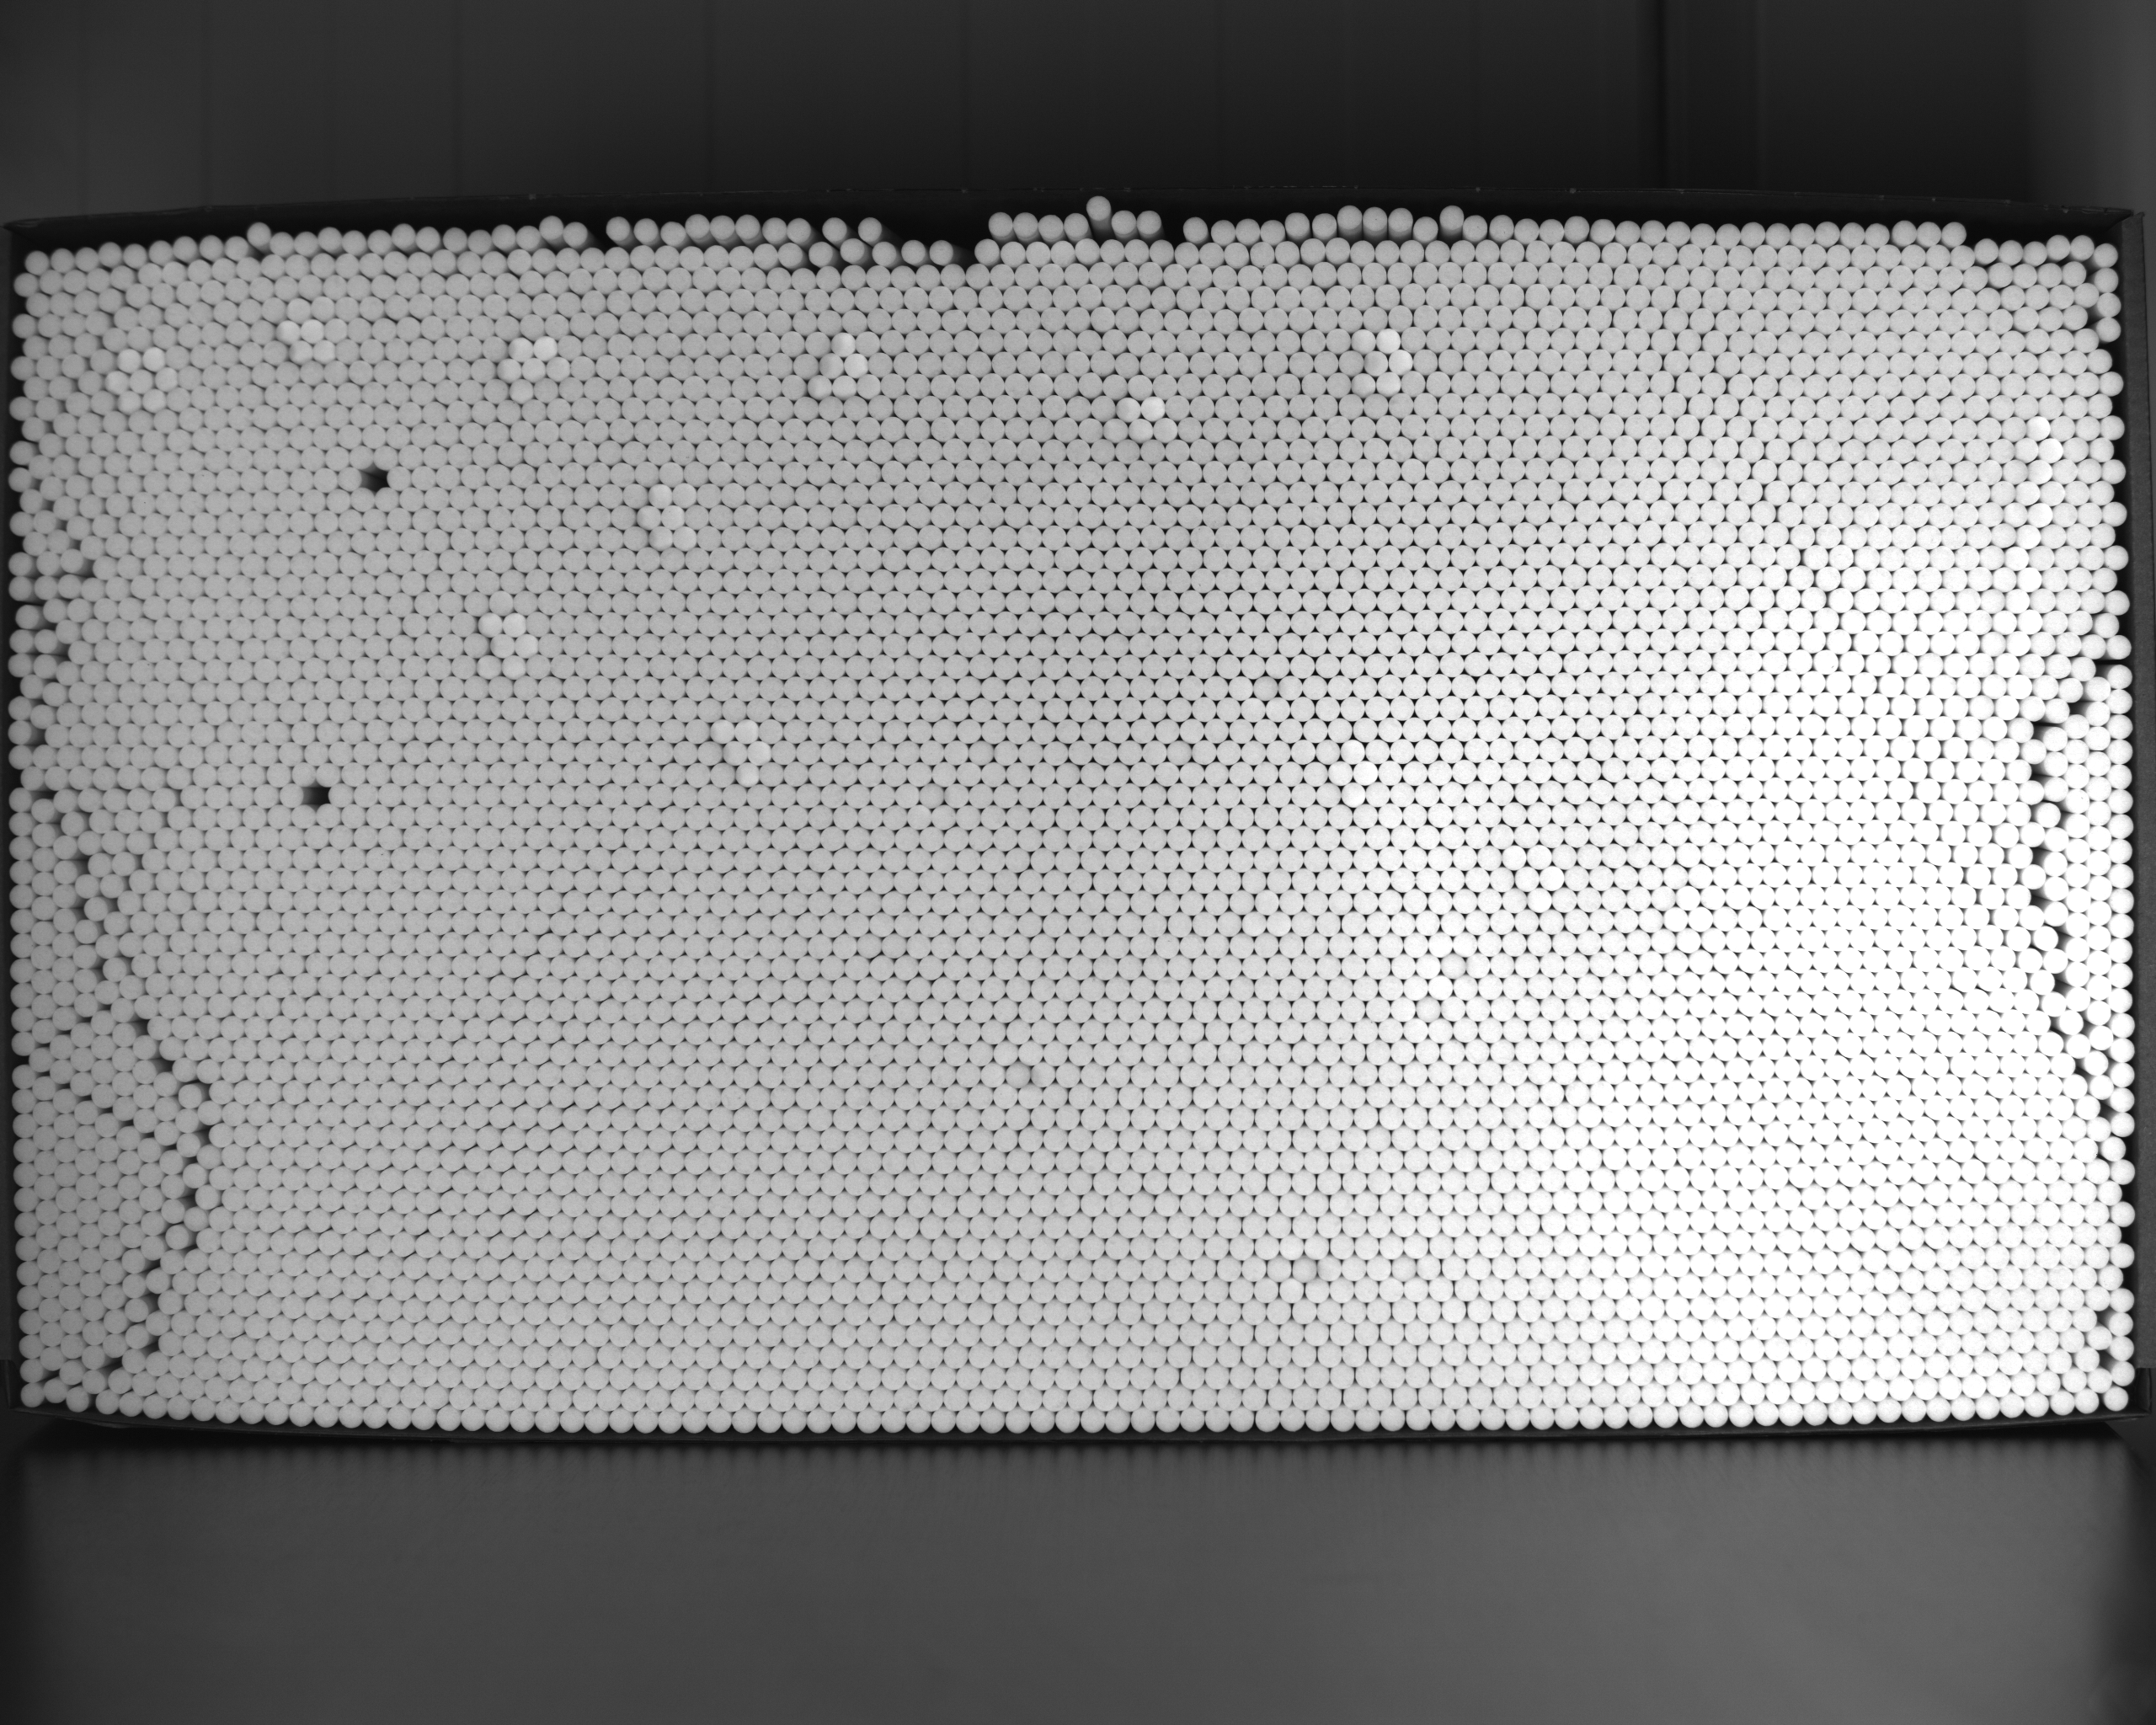
\includegraphics[scale=0.23]{3.png}}%
\qquad
\subfigure{%
\includegraphics[scale=0.0828]{circles3.png}}%
\caption{Wynik dla obrazu z nierównym oświetleniem}
\label{light}
\end{figure}

Wartym uwagi jest fakt, że dla dużych obrazów wejściowych $2560\times2048$ algorytm kończy swoje obliczenia w zaledwie $1.2s$. Szybki czas wykonania wraz z dużą dokładnością sprawiają, że program mógłby z powodzeniem zostać użyty w zastosowaniach przemysłowych.

\end{document}